\section{Open hardware, reproducibility, and cost}\label{sec:openhw}

Only about a quarter of the analyzed studies shared their design files or code. Those that did used GitHub, OSF, Zenodo, figshare, and design-sharing platforms,\citep{wittbrodt2015open,feng2021open,bulusu2024technical,stevens2024low,bogucki2019d,grasse2015teaching} or supplied the files with the article,\citep{prairie2020accurate,nonno2022portuino,delmonache2025multipurpose,yu2023open} in some cases including optical components that others can adapt.\citep{zhang2013open} The review of freshwater sensors likewise found that design files were rarely available.\citep{cirrone2026analytical}

Being able to download the files is only a start: reuse also depends on how complete they are and how they are licensed.\citep{wenzel2023open} EOSpec, for example, pairs MIT-licensed software with a noncommercial Creative Commons license for the remaining materials,\citep{feng2021open} and another instrument uses CERN-OHL-S for the hardware and separate terms for software and documentation.\citep{moralesguerra2026low} Files available only on request,\citep{glotz2018design,markvart2020continuous} or an application released without its source code,\citep{hosker2017demonstrating} leave far fewer routes to modifying and rebuilding an instrument.

\subsection{Rebuilding and calibration transfer}

Every rebuilt instrument needs its own evaluation of response. Two LED units differed in their sensitivity to iron, which the authors attributed to differences in component performance; source intensity and blank voltage also affected the calibration.\citep{prairie2020accurate} Five C12880MA spectroradiometers were characterized one by one, with shared corrections offered as an alternative.\citep{troscianko2023osprad} Two encapsulated AS7265x units gave mean readings of 13\,019.59 and 36\,185.52 counts for the same empty tank, and each needed its own model.\citep{stevens2024low} Switching phone models or reassembling an attachment brought further changes in response.\citep{bruininks2022inexpensive,vidal2021use}

Calibration data and processing records help to disentangle the effects of construction from those of analysis choices.\citep{troscianko2023osprad,moralesguerra2026low,stevens2023development,prairie2020accurate} The nitrate analyzer derived from the open-source C12880MA instrument shows how a shared design can be adapted and then evaluated for a new application.\citep{bulusu2024technical,laganovska2020portable} We intend the files we provide for systems A and B to be used in the same way: a rebuilt unit should be recalibrated and evaluated before use.

\subsection{Reading reported costs}

Figure~\ref{fig:costres} plots the numerical cost totals counted in Table~\ref{tab:valpractice}, with one marker per publication. Most are totals for a complete device or the sum of its components; the rest refer to phone attachments, sensor boards alone, or larger systems. The stars mark our systems A, B, and C, using component totals for A and B and the retail price for C.

Most totals were originally given in US dollars, and the rest in euros, pounds sterling, or Singapore dollars, in publications dated between 2015 and 2026. The original currencies, exclusions, and source evidence are kept in the extraction records. Since the dates of the prices were stated inconsistently, a common display currency does not imply equivalent purchasing conditions.

\begin{figure}[!htbp]
\centering
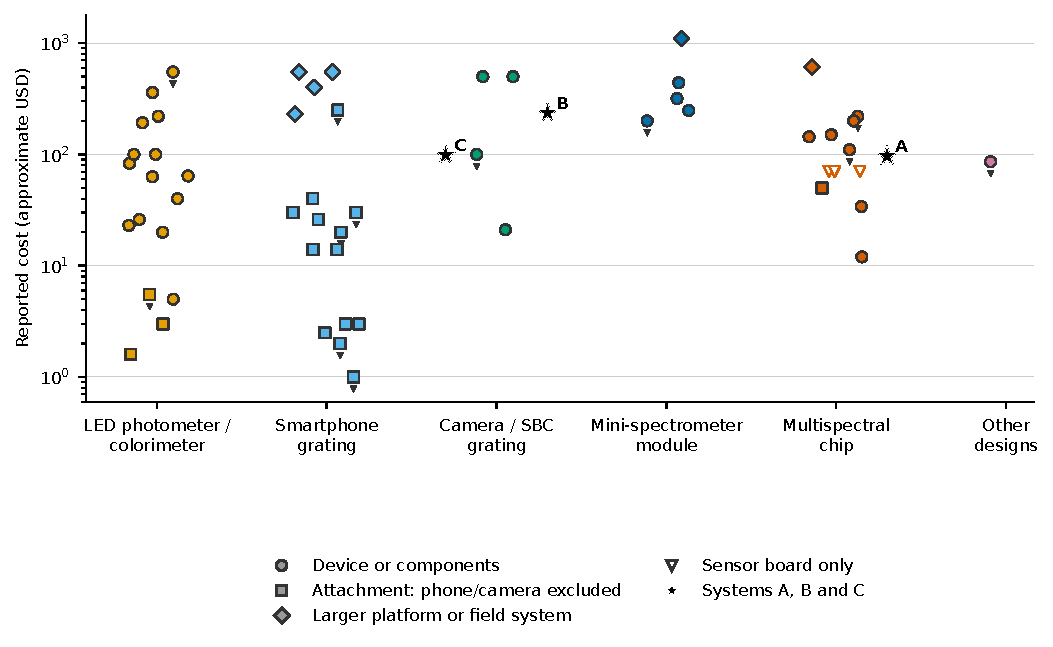
\includegraphics[width=\linewidth, draft=false]{cost_channels.pdf}
\caption{\FigureCaptionSeven}\label{fig:costres}
\end{figure}

Much of the spread comes down to what each price includes. Attachment prices leave out the phone or camera,\citep{koohkan2020fabrication,rani2021polynomial,ju2020fabrication,feng2021open} and sensor-board prices of USD~28--70 leave out the rest of the acquisition assembly.\citep{stevens2023development,stevens2024low,lopin2025evaluation} Three reports on larger systems were unclear about whether the phone was included,\citep{wang2016smartphone,long2017multimode,woodburn2019analysis} while others priced a reader together with its phone, a spectral camera, or a field analyzer.\citep{kong2020novel,sutherland2024synchronising,bulusu2024technical}

The shared designs show just how different these budgets can be: a USD~63 analog photometer,\citep{prairie2020accurate} a USD~26 freshwater photometer,\citep{cirrone2025low} the USD~30 EOSpec,\citep{feng2021open} and the EUR~225 C12880MA instrument along with its USD~1100 field adaptation.\citep{laganovska2020portable,bulusu2024technical} Teaching hardware below USD~100, a USD~50 handheld spectrometer, and a USD~144 horticultural sensor are further examples.\citep{delmonache2025multipurpose,yu2023open,moralesguerra2026low} Lists of component prices\citep{nguyen2025portable} and prices of individual printed optical mounts\citep{davis2018open} give partial information, but no instrument total that could be plotted.

Cost estimates also differ in the equipment they leave out,\citep{wang2015build} in whether they count parts only,\citep{prairie2020accurate} in whether they include reagents or fabrication,\citep{liao2020portable,habibullah2020cost} and in whether they assume manufacturing or market prices.\citep{aquino2022preliminary,kitic2019new} For an estimate to be useful to someone rebuilding the instrument, it therefore needs a dated bill of materials, a list of exclusions, the cost of assembly and calibration, and recurring expenses. These prices and channel or pixel counts are so heterogeneous that they cannot support a comparison of analytical performance per dollar.
